\documentclass{ieeeaccess}
\usepackage{cite}
\usepackage{amsmath,amssymb,amsfonts}
\usepackage{mathtools}
\usepackage{algorithmic}
\usepackage{graphicx}
\usepackage{textcomp}
\usepackage{caption}
\usepackage{subcaption}
\usepackage{float}
\usepackage[flushleft]{threeparttable}
\usepackage{bm}
\usepackage[inline]{enumitem} 
% \usepackage{amsmath}
% \usepackage{amsfonts}
% \usepackage{amssymb}
% \usepackage{fontspec}
% \setmainfont{TeX Gyre Termes}
\setcounter{MaxMatrixCols}{30}
\providecommand{\U}[1]{\protect\rule{.1in}{.1in}}
\newtheorem{theorem}{Theorem}
\newtheorem{acknowledgement}[theorem]{Acknowledgement}
\newtheorem{algorithm}[theorem]{Algorithm}
% \newtheorem{axiom}[theorem]{Axiom}
\newtheorem{case}[theorem]{Case}
% \newtheorem{claim}[theorem]{Claim}
\newtheorem{conclusion}[theorem]{Conclusion}
% \newtheorem{condition}[theorem]{Condition}
% \newtheorem{conjecture}[theorem]{Conjecture}
\newtheorem{corollary}[theorem]{Corollary}
% \newtheorem{criterion}[theorem]{Criterion}
\newtheorem{definition}[theorem]{Definition}
% \newtheorem{example}[theorem]{Example}
% \newtheorem{exercise}[theorem]{Exercise}
\newtheorem{lemma}{Lemma}
\newtheorem{notation}{Notation}
\newtheorem{problem}[theorem]{Problem}
% \newtheorem{proposition}[theorem]{Proposition}
\newtheorem{remark}{Remark}
\newtheorem{solution}[theorem]{Solution}
% \newtheorem{summary}[theorem]{Summary}
\newtheorem{assumption}{Assumption}[section]
\newtheorem{ramark}{Remark}[section]
\newenvironment{proof}[1][Proof]{\noindent\textbf{#1.} }{\ \rule{0.5em}{0.5em}}
\def\BibTeX{{\rm B\kern-.05em{\sc i\kern-.025em b}\kern-.08em
    T\kern-.1667em\lower.7ex\hbox{E}\kern-.125emX}}
    
\begin{document}
% \captionsetup[figure]{labelfont={bf},labelformat={default},labelsep=period,name={Fig.}}
% \history{Date of publication xxxx 00, 0000, date of current version xxxx 00, 0000.}
% \doi{10.1109/ACCESS.2017.DOI}

% \title{Preparation of Papers for IEEE ACCESS}
% \author{\uppercase{First A. Author}\authorrefmark{1}, \IEEEmembership{Fellow, IEEE},
% \uppercase{Second B. Author\authorrefmark{2}, and Third C. Author,
% Jr}.\authorrefmark{3},
% \IEEEmembership{Member, IEEE}}
% \address[1]{National Institute of Standards and 
% Technology, Boulder, CO 80305 USA (e-mail: author@boulder.nist.gov)}
% \address[2]{Department of Physics, Colorado State University, Fort Collins, 
% CO 80523 USA (e-mail: author@lamar.colostate.edu)}
% \address[3]{Electrical Engineering Department, University of Colorado, Boulder, CO 
% 80309 USA}
% \tfootnote{This paragraph of the first footnote will contain support 
% information, including sponsor and financial support acknowledgment. For 
% example, ``This work was supported in part by the U.S. Department of 
% Commerce under Grant BS123456.''}

% \markboth
% {Author \headeretal: Preparation of Papers for IEEE TRANSACTIONS and JOURNALS}
% {Author \headeretal: Preparation of Papers for IEEE TRANSACTIONS and JOURNALS}

% \corresp{Corresponding author: First A. Author (e-mail: author@ boulder.nist.gov).}
% .

% \begin{abstract}

% \end{abstract}

% \begin{keywords}
% Enter key words or phrases in alphabetical 
% order, separated by commas. For a list of suggested keywords, send a blank 
% e-mail to keywords@ieee.org or visit \underline
% {http://www.ieee.org/organizations/pubs/ani\_prod/keywrd98.txt}
% \end{keywords}

% \titlepgskip=-15pt

% \maketitle

\section{Introduction}
% unmanned vvehcile
\PARstart{I}{n} recent years, the unmanned vehicle (UV) has attracted attention due to the advances in communication technology, sensing devices, and computing power. It not only reduces labor costs and brings convenience to life, but more importantly, it can replace some dangerous jobs for humans. Due to these benefits, it has been widely used in many scenarios, such as search and rescue, battlefield, logistics and transportation, and surveillance, etc (cite:UV). Compared with a single UV, multiple UVs can perform more complex tasks and are more robust due to a large number of agents (cite:MAS). However, the cost is that the design of such a multi-agent system becomes more intricate as there are more problems to be resolved, such as formation, collision avoidance between agents, and cooperation between agents. In addition to the number increasment, a heterogeneous multi-agent system (HMAS) combining various types of UV is also valued (cite:HMAS). Compared with homogeneous multi-agent system, it can adapt to a wider variety of application scenarios. Although there are many types of UVs to make up such a system, Unmanned Aerial Vehicle (UAV) and Unmanned Ground Vehicle (UGV) have been the subject of major recent research because of their availability and applicability (cite:UAV-UGV). Additionally, the complementarity between them also makes such a system more potential. In other words, UAV is widely used in reconnaissance due to the high mobility. However, the carrying capacity of UAV is very low compared to UGV since there is no ground support. In contrast, UGV has higher carrying capacity but is easily restricted by ground obstacles and cannot move at high speed. For these reasons, a hybrid UAV-UGV system will be more practical.

To construct an unmanned HMAS, it must be capable of perception, decision-making and execution. Perception is to obtain information through the sensor, decision-making is to make decisions through the sensor information, and execution is to execute the decision-making content through the actuator. To limit the scope of this paper, we focus on decision-making and execution for an UAVs-UGVs search and rescue system.

The four more specific main problem in decision-making and execution are task allocation problem (cite: task allocation), path planning problem (cite: path planning), local motion planning problem and tracking control problem. These four problems form a hierarchical structure in order. First, the UAVs-UGVs search and rescue system needs to be able to assign different tasks to agents to perform. After a task is assigned, if the task is to reach a target location, a path needs to be planned to reach it. To make agent move on the path, a motion corresponding to the actual mechanical system of the agent needs to be planned. Finally, a controller must be designed to track the trajectory of the motion. In order to further limit the scope of the study, we will focus on the latter two problems. But to illustrate how the whole system works, the first two problems are also briefly stated.
% An unmanned search and rescue system needs to be able to assign different tasks to agents to perform. This problem is called the task allocation problem, which attempts to achieve an optimal allocation given the objective function and some constraints (cite: task allocation). After a task is assigned, if the task is to reach a target location, a path needs to be planned to reach it. This problem is called the path planning problem, which attempts to achieve an optimal path given the objective function and some constraints (cite: path planning).

To discuss the local motion planning problem and tracking control problem, a real mechanical system to which each agent corresponds must be considered. To meet the need for search mobility, we choose quadrotor aircraft as UAV. The control problem of UAV has been widely studied due to its applicability and low cost (cite: uav control). In order to deal with the complex terrain of the search and rescue environment, biped robot was chosen as the UGV. Although other types of UGVs like wheeled robots and vehicles are easier to handle than biped robot, the high degree of freedom and the compatibility of the human environment still makes it a good candidate of UGV in a search and rescue system. However, to let the biped robot moving, not only the control problem (cite: robot control) but also the local motion planning problem need to be solved. The local motion planning of the walking of biped robot, i.e., stable walking parttern generation, is discussed in this paper. Related researches can be found in (cite: walking parttern).

The local motion planning is the bridge between path planning and tracking control since the path found by path planning algorithm and the path enforced to follow by a controller are not necessarily the same. The reason is that path planning algorithm usually treats the agent as a point, while the actual agent is a mechanical system for the tracking control design. Although there are some literatures (ref:kinodynamic path planning) about path planning with the constraints of kinodynamic of the actual mechanical system, this paper splits it into three steps, i.e., (i) path planning, (ii) behavior layer and (iii) local motion planning for clarity.
% The aforemention two problems are widely studied in the field of computer science and field of control respectively but fewer papers point out their relationship with respect to specific agents (UAV and robot in this paper). Therefore, this paper will focus on this issue.

Tracking Problem ...

To the best of the authors' knowledge, most of the literature focus on only one specific problem, and few literatures illustrate the relationship between these problems for an unmanned HMAS. This leads us to propose an architecture of UAV-robot team system (URTS) for search and rescue although this paper mainly focuses on the local motion planning and tracking control problem.
% Based on the foregoing, an UAV-robot team system (URTS) is discussed in this paper.

% \PARstart{W}{ith}

The contributions of this study are described as follows:
\begin{enumerate}
    \item contribution 1 ...
\end{enumerate}

The remainder of the paper is organized as follows. In Section II, ...

\textbf{Notation 1:} 
% $diag(A_1, A_2, \dots, A_n)$: a block diagonal matrix with main diagonal blocks $A_1, A_2, \dots, A_n$.
$A^T$: transpose of A. $(a_n)$: sequence. $(a_{k_n})$: subsequence. $\vert{S}\vert$: size of a set $S$. $\otimes$: Kronecker product. $I_n$: n-dimension identity matrix. $x(t)\in L_2\begin{bmatrix}
    0,t_f 
\end{bmatrix}$ if $\int^{t_f}_{0}x^T(t)x(t)dt<\infty$.

\section{PRELIMINARIES OF search and rescue URTS}
The URTS will start with a given search and rescue area, and ends with searching task completed. The URTS is composed of $N$ teams and a ground station. Each team contains $1$ UAV and $M-1$ robots. The $i$th agent in the $j$th team is denoted as $agent_{i,j}$, where $i=1,2,...,M$ and $j=1,2,...,N$. The UAVs are chosed as the first agents in each team, i.e., $agent_{1,j}$. Each agent has environmental sensing capability and load capability, while the ground station is responsible for computing and decision-making. Besides, there are communication channels between agents and ground station through wireless network.
% The system architecture if URTS is shown in Fig. \ref{fig:1}.
% \begin{figure}[htbp]
% \centering
% 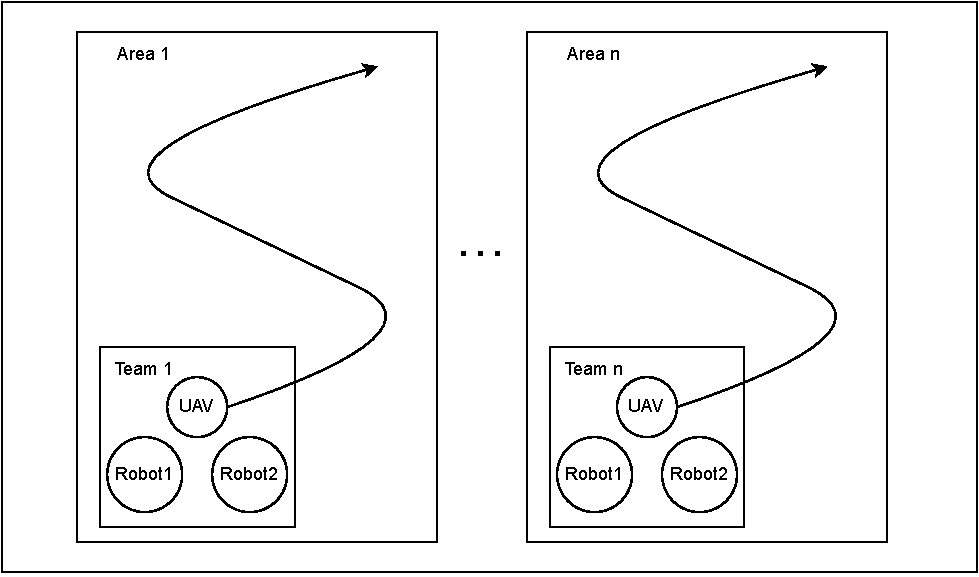
\includegraphics[width=0.4\textwidth]{fig/1.pdf}\caption{System structure of URTS}%
% \label{fig:1}
% \end{figure}

To complete search tasks, each team is designed to be responsible for a small area of the overall search area, and each agent will be assigned an appropriate path to cover the area. To complete rescue tasks, whenever a target (e.g., victims or disaster area) is found by the machine vision of nearby agent, the ground station will assign some agents to the location of target. It can be expected that there has multiple search or rescue tasks need to be performed at the same time but there has multiple agents. If each agent can only perform one task at a time, then there exist many feasible way of task allocation. Usually we want this allocation to be optimal, which can be achieved by solving the dynamic task allocation problem.

If a task is to reach a location of certain goal, there must exist multiple feasible paths. Similar to task allocation, we usually want to find an optimal path. Besides, it's necessary to concern about collision between agents or between agents and obstacles in the actual scenario, so each agent will also sense distance-related information about its surrounding and send it back to the ground station. The ground station will combine this information with the goal assigned by task allocation algorithm and make a decision to avoid obstacles and other agents nearby. That is, the path of each agent will be reassigned every moment if needed by solving the dynamic path planning problems.

We need to design some behavior to follow the path found by path planning algorithm especially for agents with complex mechanical systems like robots. Since such a system has a high degree of freedom, there are many ways to follow the same path (e.g., a robot can walk or run to follow the same path). Furthermore, agents in a search and rescue system are not always following a trajectory. Sometimes they need the behavior such as stop to look around, get supplies and put supplies. To meet these needs, a behavioral layer is necessary. The behavior layer gives an appropriate behavior to fulfill an actual requirement. In order to make an behavior, we must design a corresponding motion which is handled by local motion planning. The motion is a desired reference trajectory for an actual mechanical system to follow. Finally, a tracking controller is designed to follow the desired reference trajectory.

To clarify this issue, a more detailed system architecture for each agent is needed. Followed by the concept in \cite{paden2016survey}, a system architecture for an agent used in search and rescue is proposed as shown in Fig. \ref{fig:sys}. The Simultaneous Localization And Mapping (SLAM) block converts sensor information into the location of agents and an occupy map. The visual object recognition block provides distance information and object information through sensor info. The object information provides agent machine vision that enables it to determine an appropriate behavior (e.g., a robot sees a obstacle and decides to climb through it). The detailed functions of remaining 5 blocks, i.e., Tack Allocation, Path Planning, Behavior Layer, Local Motion Planning and Tracking Control, will be explained in the following sections.

% To determine the behavior, agent needs the information about enviroment. The sensing data which include external enviroment information and internal system information is feedback to Behavior Layer to assist in judging the present state (fig:system). 

\begin{figure}[htbp]
\centering
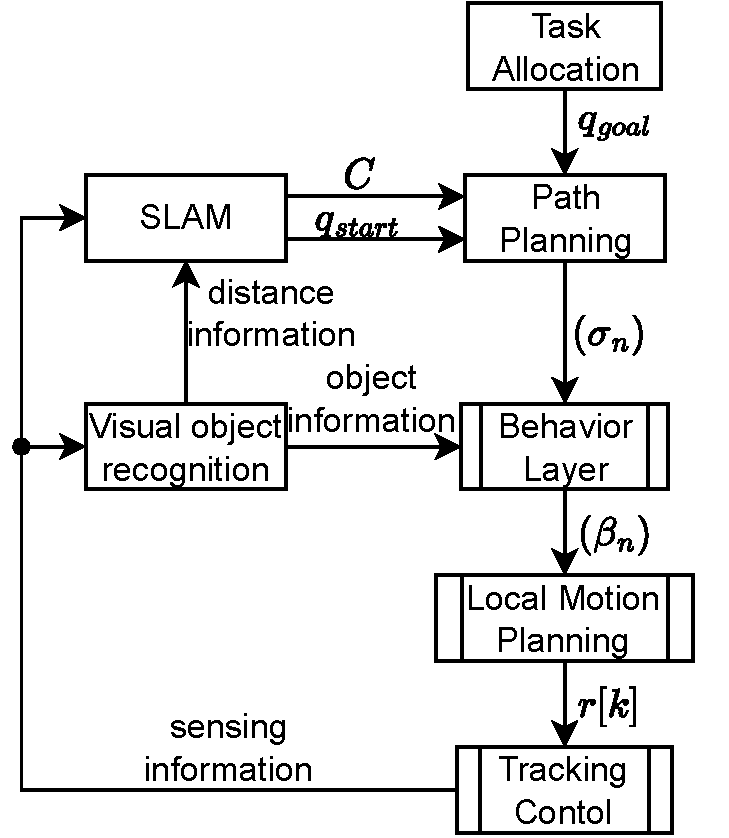
\includegraphics[scale=.5]{fig/sys.pdf}\caption{The system architecture of agent in URTS. The 2 blocks on left side are used to convert low-level sensor information into high-level information, such as map, start point and object information. The 5 blocks on right side are the flow of an agent performing a search and rescue mission. From top to bottom, it is the decision of the task position, the planning of the path, the decision of the behavior, the planning of the local motion trajectory, and the low-level tracking control}%
\label{fig:sys}
\end{figure}

\subsection{Task Allocation}
In the URTS, it can be expected that each agent will be assigned several specific tasks, such as searching a specific area, or delivering supplies to disaster area, etc. However, the number of agent and task is more than one, and each agent has different capabilities (e.g. moving speed or load capacity) and status (e.g. their own position or the amount of supplies carried), and each task has different characteristics (e.g. Urgency, position, amout of supplies needed). Therefore, the results of task allocation can be "good or bad", which makes us want to find the optimal allocation. This problem is refered as Task Allocation Problem or Multi-robot Task Allocation (MRTA) Problem. A problem formulation and problem modeling can be found in \cite{Khamis2015}. Although there are many different problem definitions and many problem models to solve this issue, the common goal is to find a set of task-agent pairs to achieve a specific cost function. In this paper, we assume that the tasks have been properly assigned and therefore do not further discuss this issue. In other words, every agent knows a destinition it need to go at every moment.
% $(\mathcal{G})_n, n\in\mathbb{Z}\cap[1, N], N\in\mathbb{Z}^+$
\textit{
    \begin{remark}
        This block is like a commander since it is used to assign task for agents. Thus, if the real search and rescue system has human experts as commanders, he can replace its job or make decisions together with it to maximize the rescue value.
    \end{remark}
}

\subsection{Path Planning}
After a target point is assigned for each agent, next step is to find a collision-free path from current position to it. There are several path planning algorithm to handle this problem, in this article, a roadmap-based path planning algorithm is used. This method attempts to discretize the search space into interconnected roads and find the path on it. According to the roadmap construction method, it can be divided into deterministic and sample-based. According to the way of pathfinding, it can be divided into multi-query planner and single-query planner \cite{elbanhawi2014sampling}. Multi-query planner divides pathfinding into learning phase in which a roadmap is bulit and query phase in which a graph search algorithm is used to find a best path within paths. Some representative planners are Probability Road Map (PRM), Visibility Graph, and Voronoi Diagrams \cite{liu2018survey}. Relatively speaking, single-query planner completes pathfinding by constructing and querying at the same time, that is to say, the roadmap will be constructed incrementally and toward the goal. Some representative planners such as Rapidly-exploring Random Tree (RRT), Expansice Space Tree (EST), and Ariadne's Clew \cite{elbanhawi2014sampling}. However, the environment is dynamic rather static for URTS so some extra structure need to impose on aforementioned planner. Some common dynamic planner also can be found in \cite{elbanhawi2014sampling}, such like PRM with D* search algorithm, dynamic RRT, and extended RRT.

Furthermore, the constraints imposed by the mechanical structure are needed to consider within pathfinding process mentioned by other literatures but it will be left to Local Motion Planning to deal with. The reason is that URTS is a large-scale system, which makes the environment in which it is located changes more violently and will leads to many corresponding behaviors which path constraints will not necessarily be the same (e.g., curvature constraints of two behavior: running and walking are expected to be different for robot). In this case, Path Planning becomes a higher-level planner which regard agent as a point without kinodynamic constraints while the decision of the behavior and the corresponding motion will be handed over to the next two layers: Behavior Layer and Local Motion Planning.
% In this case, the configuration space $\mathcal{C}$ degenerates to $\mathbb{R}^3$.

By treating a roadmap-based path planning algorithm as a black box, the output is a sequence (or sayed waypoints), and the three inputs are current configuration $q_{start}$, goal configuration $q_{goal}$, and configuration space $\mathcal{C}$. Current configuration is obtained by GPS, inertial measurement unit, or other locating techniques. Goal configuration is obtained by previous layer: Task Allocation. Configuration space $\mathcal{C}$ is constructed by environment information through sensors of agents online or in advance by human knowledge offline. It's a space contain all possible configuration of agent which composed of free space $\mathcal{C}_{free}$ and obstacle space $\mathcal{C}_{obs}$, where $\mathcal{C}=\mathcal{C}_{free}\cup\mathcal{C}_{obs}$ and $\mathcal{C}_{free}\cap\mathcal{C}_{obs}=\emptyset$. For a simpler explanation of how the URTS works, the following assumption is made.
\begin{assumption}
    The locating ability of the URTS is perfect so every agent can know its current configuration $q_{start}$.
\end{assumption}
\begin{assumption}
    A Task Allocation algorithm is already designed so that every agent can know its goal configuration $q_{goal}$.
\end{assumption}
\begin{assumption}
    The URTS is supposed to have an perfect real-time mapping ability so a real-time configuration space $\mathcal{C}$ can be obtain.
\end{assumption}
\begin{assumption} \label{asm:collision}
    UAVs do not consider obstacle collisions because there are few obstacles in the air. Hence, the path of UAVs can be directly assigned rather found by planner. Robots do not consider obstacle collisions in the direction perpendicular to the ground. 
\end{assumption}
From above assumption, a path of agent can be expressed as a sequence
\begin{equation}
    (\sigma_n), n\in\mathbb{Z}\cap[1,k_f], \sigma_n\in\mathcal{C}
\end{equation}
where $k_f$ is the time step when reaching goal. Since the path planning is dynamic, $(\sigma_n)$ is composed of multiple segments actually. Let $(\sigma_{k_n})$ be the subsequence of $(\sigma_n)$, where $k_n$ is the time step when a replanning decision is occured. Then, the segments of path from the result of the replanning in time step $k_n$ can be expressed as sequences $(\sigma_m), m\in\mathbb{Z}\cap[k_n, k_{n+1})$. For agents, the replanning decision can be a goal changing that made by human or Task Allocation. For robot, it can be a collision detecting by a dynamic roadmap-based planner. The results path $(\sigma_n)$ is passed to next layer, Behavior Layer.

\subsection{Behavior Layer}
% Since UAVs and robots are real physical systems, they must interact with the environment through a behavior so that they can move and act in the physical world.
Path Planning tells agents where to go but not how. Take robot as an example, it may walk, run, climb, or jump to follow the path $(\sigma_n)$ in real scenario. These behaviors with changing position are called "moving" in this paper. Besides, the agents do not always moving. Somtimes they has to suspending to take a action such like getting and putting supplies, rotating in place to collect more environment info, or some unexpected situations occur such like no path found, the robot falls. These behaviors without changing position are called an "action" in this paper. More behaviors can be added so that the agent can have more way to act with environment but there must have a corresponding behavior every moment otherwise the agent will lose control. The sequence of these behaviors be expressed as:
\begin{equation}
    (\beta_n), n\in\mathbb{Z}\cap[1,k_f], \beta_n\in\mathcal{B}
\end{equation}
It is to say that the path $(\sigma_n)$ is divided into many segments which corresponding to a specific behavior. The set of behavior $\mathcal{B}$ of agent in URTS can be roughly discribed in Fig. \ref{fig:behavior}.

\begin{figure*}[htbp]
    \centering
    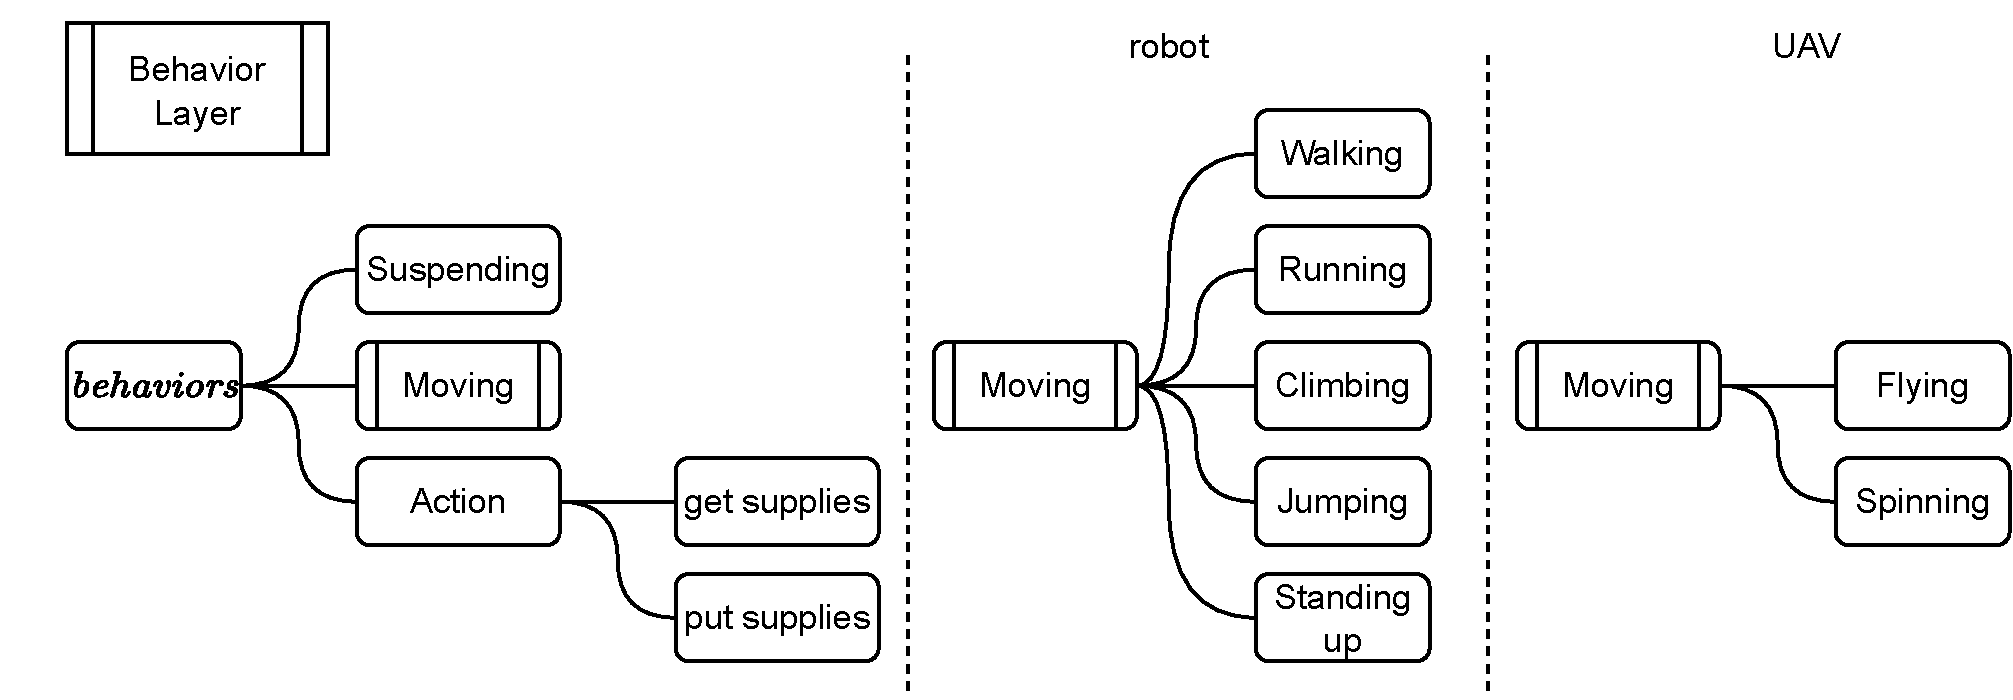
\includegraphics[scale=.5]{fig/behavior.pdf}\caption{The structure of Behavior Layer. The leaf of the tree structure are the possible behaviors an agent can take. The behavior to be take at every moment will be decided in this block.}%
    \label{fig:behavior}
\end{figure*}

\subsection{Local Motion Planning}
After a specific behavior is determined, the next step is to design a motion to achieve that behavior. Local Motion Planning is like Path Planning but its scale is smaller and its resolution and precision must be higher. Collision checking is needed since we consider agent as a point or a cube in Path Planning and it's a real body here. Furthermore, the kinodynamic constraint is handled in this block. Although motion planning and path planning are separated into two blocks, the technologies involved are similar and often the same notion in other literature. Therefore, the output of this block is also a path but with a sampling period which often be referred as a reference trajectory $r(t)$. $r(t)$ describes the position and orientation that needed to be reach by a machine system govern by a dynamic equation. Then, Tracking Control block will track $r(t)$ to really do that behavior. Note that the path and trajectory are distinguished in some literature. Different from path (e.g., $(\sigma_n)$), a trajectory (e.g., $r(t)$) has consider the time in physic world. The flowchart of Local Motion Planning block is shown in Fig. \ref{fig:LocalMotionPlanning}

\begin{figure*}[htbp]
    \centering
    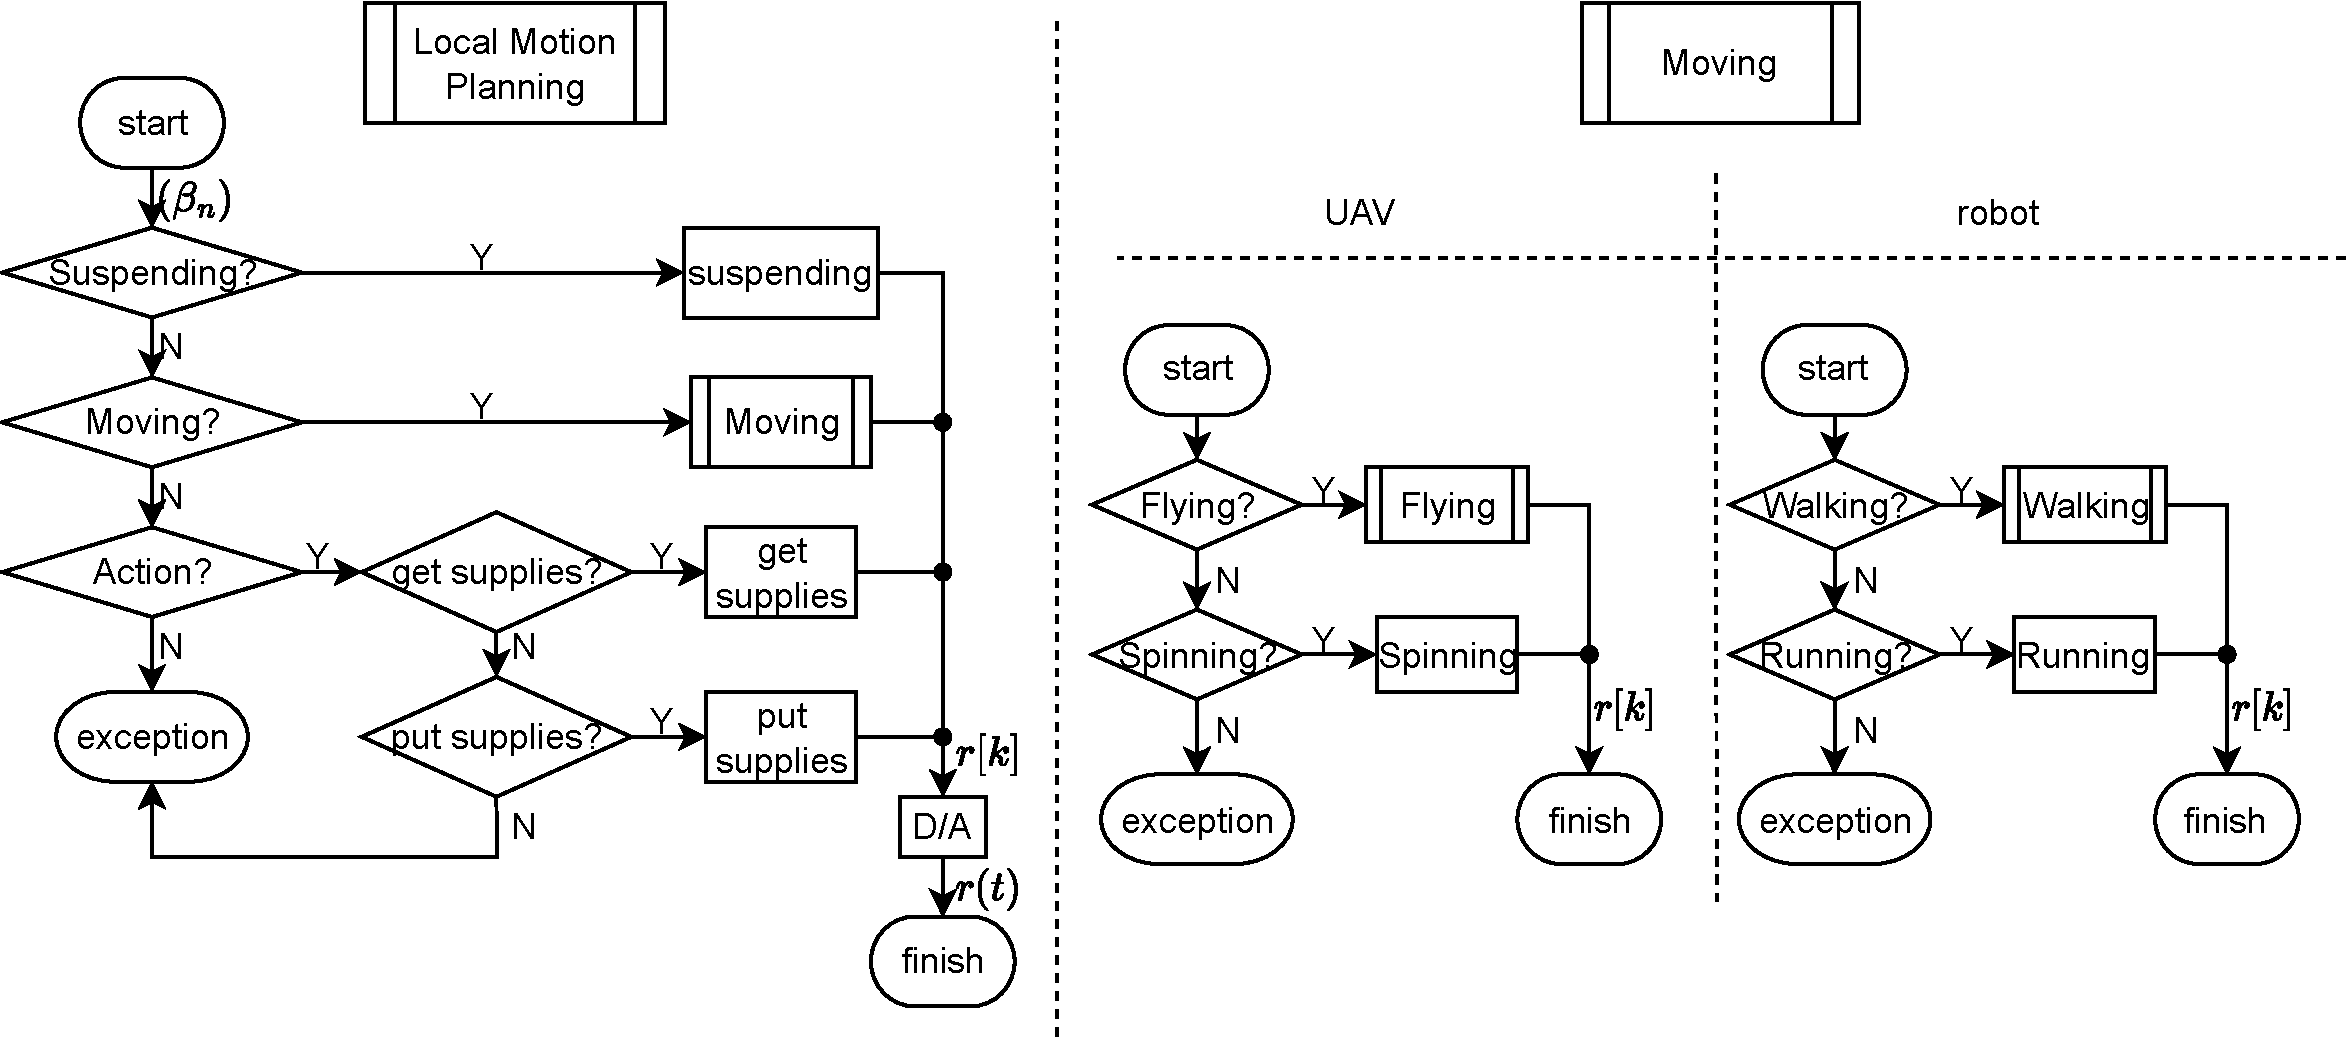
\includegraphics[scale=.4]{fig/LMP.pdf}\caption{The flowchart of local motion planning. The corresponding motion design will be executed according to the behavior determined by the behavior layer.}
    \label{fig:LocalMotionPlanning}
\end{figure*}

In Fig. \ref{fig:LocalMotionPlanning}, some basic behaviors of UAV and robot mentioned before are added to illustrate the flow of this block. The terminator, exception, represents an exceptional condition that performs unconsidered behaviors. To limit the scope of this article, we only focus on the motion design of Flying (for UAV) and Walking (for robot) behavior which belong to Moving behavior. The reference path $r[k]$ is a sequence (or say a discrete signal) designed by a specific behavior block. It then convert to reference trajectory $r(t)$, an analog signal, by an A to D convertor.

\section{system description of UAV-Robot Team System}
In order to design a reference trajectory $r(t)$ for the motion of UAV and robot, their dynamic models must be given first. After the system description of UAV and robot, the motion design of Flying and Walking as shown in Fig. \ref{fig:FandW} will be discussed subsequently and separately in the next two subsections.

\begin{figure*}[htbp]
    \centering
    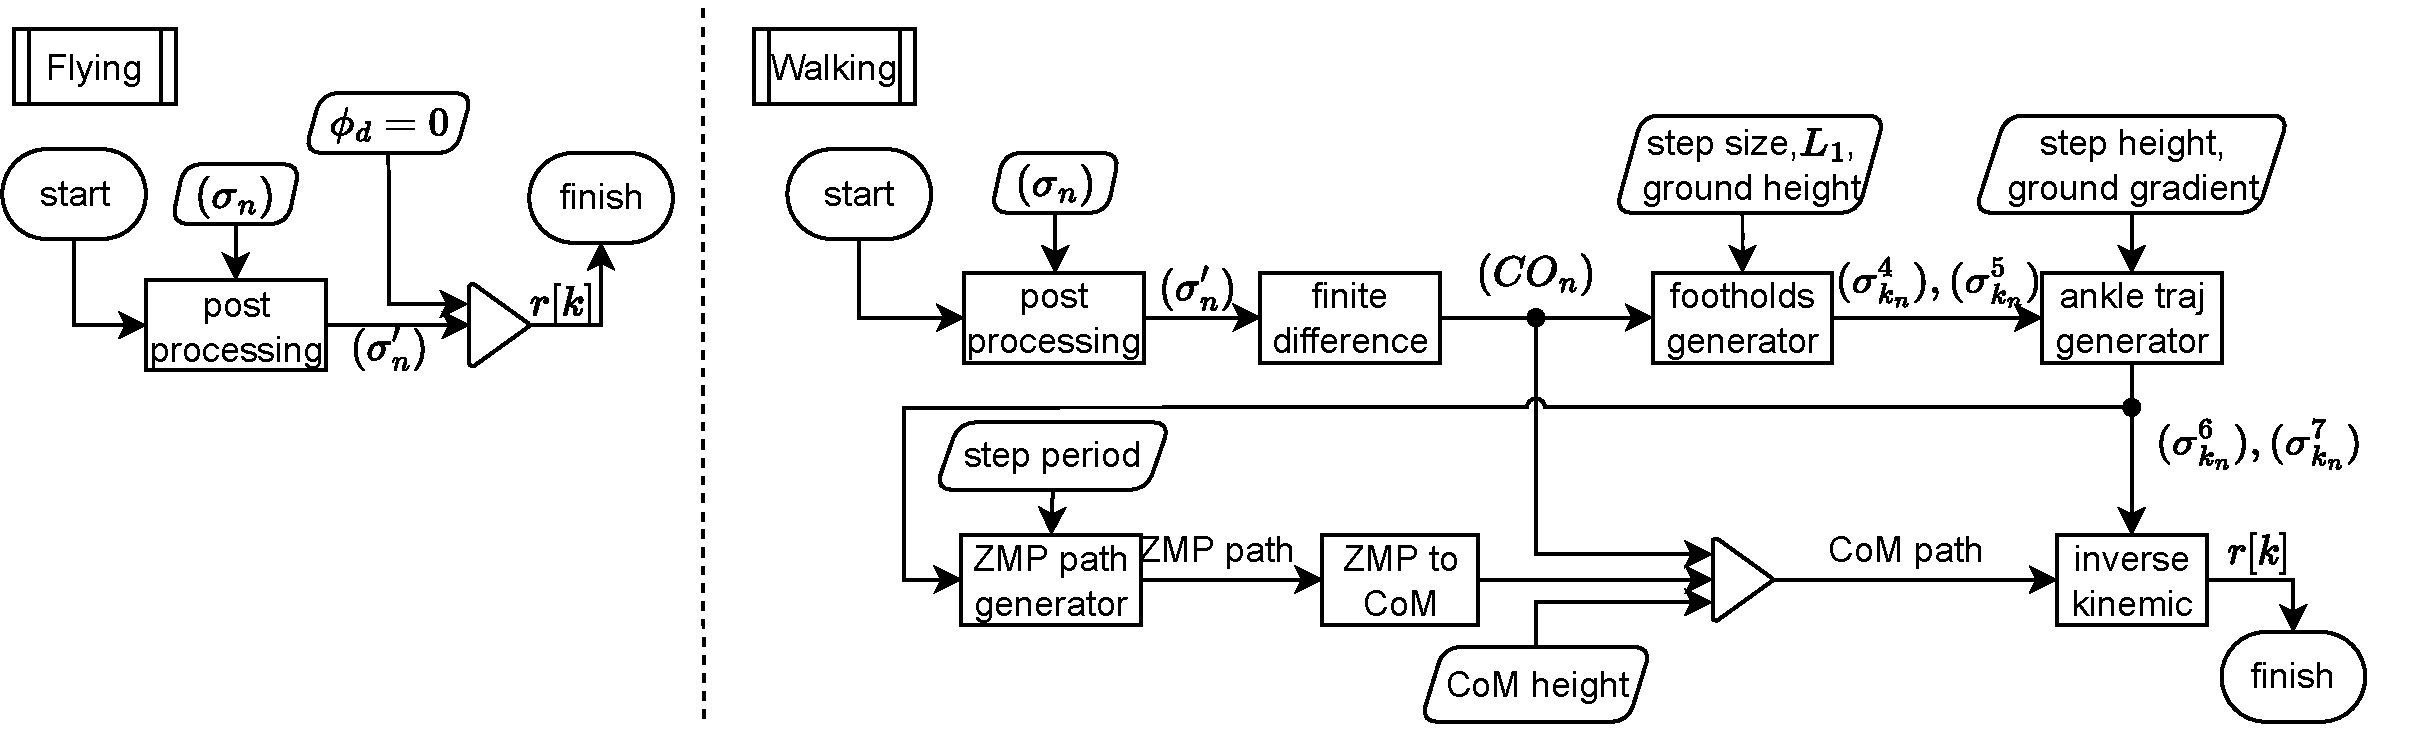
\includegraphics[scale=.4]{fig/FandW.pdf}\caption{The flowchart of Flying and Walking. In both two blocks, a smoothed path is obtained by post-processing first. Then the respective motion of behavior is designed. The final output is all reference path $r[k]$, but its actual size and dimensions will be different.}
    \label{fig:FandW}
\end{figure*}

Before the discussion of the motion design of these two behavior, the following assumption is maded.
\textit{
    \begin{assumption} \label{asm:cc again}
        The space between obstacles is large enough to eliminate the need for collision checking again, and the average speed of agents is slow enough to ignore dynamic constraints
    \end{assumption}
}
However, for these two behaviors, there all exists an inevitable kinematic constraint on curvature of local motion. Although an accurate reference trajectory without breaking the curvature constraint can be designed, it is not easy to solve this problem. Additionally, it is not nessasry for these two behaviors in URTS since they are uesd to move from one location to another while the effect of error during moving caused by breaking curvature constraint is relatively insignificant. At the same time, the assumption \ref{asm:cc again} makes sure the error will not causing collision. As an alternative, this problem can be handled by curve fitting which can be regarded as a post-process of the path $(\sigma_n)$. The post-process will appear in the begining of motion design process of these two behaviors as shown in Fig. \ref{fig:FandW}.

\subsection{motion design of flying of UAV}
A dynamic model about how the UAV moves in the physical world is given first. By Newton-Euler equation, the dynamic model of UAV can be formulated as \cite{sabatino2015quadrotor}:
\begin{equation} \label{eq:uav} 
    \begin{split}
        \begin{bmatrix}
            f \\ \tau
        \end{bmatrix}&=\begin{bmatrix}
            mI & 0 \\ 0 & J
        \end{bmatrix}\begin{bmatrix}
            \ddot{X} \\ \ddot{\Theta}
        \end{bmatrix}+\begin{bmatrix}
            0 \\ \dot{\Theta}\times(J\dot{\Theta})
        \end{bmatrix}+\begin{bmatrix}
            f_g \\ 0
        \end{bmatrix}
        \\
        &+\begin{bmatrix}
            K_F & 0 \\
            0 & K_\tau
        \end{bmatrix}\begin{bmatrix}
            \dot{X} \\ \dot{\Theta}
        \end{bmatrix}
        % form 2
        % &R(\Theta)=\begin{bmatrix*}[l]
        %     \cos\theta\cos\phi & \sin\phi\sin\theta\cos\psi-\cos\phi\sin\psi & R_1 \\
        %     \cos\theta\sin\phi & R_2 & R_3 \\
        %     -\sin\theta & \sin\phi\cos\theta & R_4
        % \end{bmatrix*}
        % \\
        % &R_1=\cos\phi\sin\theta\cos\psi+\sin\phi\sin\psi
        % \\
        % &R_2=\sin\phi\sin\theta\sin\psi+\cos\phi\cos\psi
        % \\
        % &R_3=\cos\phi\sin\theta\sin\psi-\sin\phi\cos\psi
        % \\
        % &R_4=\cos\phi\cos\theta
    \end{split}
\end{equation}
where $J=\begin{bmatrix}
    J_{x} & 0 & 0 \\
    0 & J_{y} & 0 \\
    0 & 0 & J_{z}
\end{bmatrix}$, $K_F=\begin{bmatrix}
    K_{x} & 0 & 0 \\
    0 & K_{y} & 0 \\
    0 & 0 & K_{z}
\end{bmatrix}$, $K_\tau=\begin{bmatrix}
    K_{\tau_x} & 0 & 0 \\
    0 & K_{\tau_y} & 0 \\
    0 & 0 & K_{\tau_z}
\end{bmatrix}$, $f =\begin{bmatrix}
    f_x \\ f_y \\ f_z
\end{bmatrix} = R(\Theta)\begin{bmatrix}
    0 \\ 0 \\ F
\end{bmatrix}$, $\tau=\begin{bmatrix}
    \tau_x \\ \tau_y \\ \tau_z
\end{bmatrix}$, $X=\begin{bmatrix}
    x \\ y \\ z
\end{bmatrix}$, $\Theta=\begin{bmatrix}
    \phi \\ \theta \\ \psi
\end{bmatrix}$, $f_g=\begin{bmatrix}
    0 \\ 0 \\ -mg
\end{bmatrix}$, $R(\Theta)=R_z(\psi)R_y(\theta)R_x(\phi)$, $R_z(\psi)=\begin{bmatrix} % form 1
    \cos\psi & -\sin\psi & 0 \\
    \sin\psi & \cos\psi & 0 \\
    0 & 0 & 1
\end{bmatrix}$, $R_y(\theta)=\begin{bmatrix}
    \cos\theta & 0 & \sin\theta \\
    0 & 1 & 0 \\
    -\sin\theta & 0 & \cos\theta
\end{bmatrix}$, $R_x(\phi)=\begin{bmatrix}
    1 & 0 & 0 \\
    0 & \cos\phi & -\sin\phi \\
    0 & \sin\phi & \cos\phi
\end{bmatrix}$.
% where $y'$ denotes the $y$ axis after rotating the $z$ axis and $x''$ denotes the $x$ axis after rotating the $y'$ axis
$m$ and $J$ is the mass and inertia matrix of UAV, respectively, $\tau$ and $f$ are the total touque and force acting on UAV, respectively, $\Theta$ is the Euler angles in body frame, $X$ is the postion of center of mass (CoM) in inertial frame, $K_\tau$ and $K_F$ are the aerodynamic damping coefficients, $R(\Theta)$ is the intrinsic rotation matrix from body frame to inertial frame, and $F$ is the total thrust. This model treats the UAV as a mass point and can control the force in the $z$ direction and the touque in the $x$, $y$ and $z$ direction. Hence, the reference trajectory of UAV $r(t)=[x_r(t),y_r(t),z_r(t),\phi_r(t),\theta_r(t),\psi_r(t)]^T\in\mathbb{R}^{6}$, where the subscript $r$ denote the reference.
% For ease of discussion later, let us convert (\ref{eq:uav}) into the following form:
% \begin{equation}
%     F_w=M(X_w)\ddot{X_w}+C(\dot{X_w})+G(X_w)+F(\dot{X_w})
% \end{equation

Now, suppose the UAV flying is occured between time step $t_1$ and $t_2$, that is, $(\beta_n)=\mathit{flying}, n\in\mathbb{Z}\cap[t_1,t_2]$. The corresponding path $(\sigma_n), n\in\mathbb{Z}\cap[t_1,t_2]$ will be smoothed by linear interpolation and spline interpolation which give the smoothed path $(\sigma_n'), n\in\mathbb{Z}\cap[t_1,t_1+D(t_2-t_1)], \sigma_n'\in\mathbb{R}^3$, where $D\in\mathbb{Z}^+$ is the interpolation density. $(\sigma_n')$ is the position reference path $\begin{bmatrix}
    x_r[k] & y_r[k] & z_r[k]
\end{bmatrix}^T$. Subsequently, the orientation reference path, row angle $\phi_r[k]$, pitch angle $\theta_r[k]$ and yaw angle $\psi_r[k]$ are set. $\phi_r[k]$ is set to zero since no need for spinning when flying. $\theta_r[k]$ and $\psi_r[k]$ cannot be set since UAV is an underactuated system, which will be discussed in the next section. Finally, the reference path $r[k]$ of UAV can be obtained by combining them together, i.e., $r[k] = \begin{bmatrix}
    x_r[k] & y_r[k] & z_r[k] & \psi_r[k]
\end{bmatrix}^T$. The flowchart is shown in Fig. \ref{fig:FandW}.

% \begin{figure}[htbp]
%     \centering
%     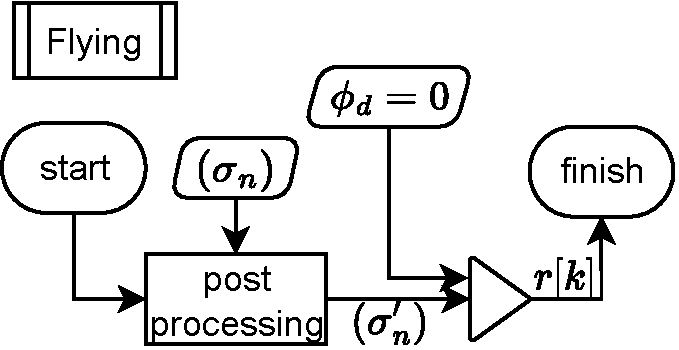
\includegraphics[scale=.5]{fig/flying.pdf}\caption{flowchart of UAV flying}%
%     \label{fig:flying}
% \end{figure}

% task space $\mathcal{T}\subset\mathbb{R}^6$.
% The terminologies, task space and joint space, are often used in reference designed in robotics. Task space is the space which the task be assigned and joint space is the space of robot joints. The forward kinematic is the mapping from joint space to task space and inverse kinematic is the inverse mapping. Since the reference of robot is in joint space ...

\subsection{motion of walking of robot}
By Lagrange equation, the dynamic model of biped robot can be formulated as:
\begin{equation} \label{eq:robot} 
    \begin{split}
        & \tau = M(q)\ddot{q} + C(q,\dot{q})\dot{q} + G(q)    
    \end{split}
\end{equation}
where $q,\dot{q},\ddot{q}\in\mathbb{R}^{12}$  are angular position, angular velocity, and angular acceleration vector of revolute joints, $M(q)\in\mathbb{R}^{12\times 12}$ is the inertia matrix, $C(q,\dot{q})\in\mathbb{R}^{12}$ is the Coriolis and centripetal force vector and $G(q)\in\mathbb{R}^{12}$ is the gravitational force vector. The detailed kinematic and dynamic parameters can be found in the online source \cite{ourrobot}. For robot, the reference trajectory $r(t)=q_r(t)\in\mathbb{R}^{12}$ is in the joint space. Furthermore, the walking of biped-robot suffers from the falling problem, i.e, how to find a stable walking parttern prevent robot from falling. These make the design of walking motion more difficult. In this paper, a three-dimensional linear inverted pendulum Mode (3D-LIPM) \cite{kajita2001real} is used to design the walking motion.

Taking the forward direction of robot as $\widehat{X_b}$ direction, the left direction as $\widehat{Y_b}$ direction, and the torso direction as $\widehat{Z_b}$ direction in body frame as in \cite{ourrobot}, "Falling" means the moments on the robot in $\widehat{X_b}$ and $\widehat{Y_b}$ direction are not zero. More accuately, the robot will not fall if the zero moment point (ZMP) lies in the support polygon which is the convex hull of face of supported foots. The ZMP in $\widehat{X_b}$ direction can be discribed as \cite{huang2001planning} ($\widehat{Y_b}$ direction as same form):
\begin{equation}
    x_{zmp} = \frac{\sum_{i=1}^{12} (m_i(\ddot{z}_i+g)x_i - m_i\ddot{x}_iz_i - I_{iy}\ddot{\Omega}_{iy})}
                   {\sum_{i=1}^{12} m_i(\ddot{z}_i+g)}
\end{equation}
It can be seen that ZMP is related to 12 link masses, moment of inertia, positions, accelerations, and angular velocities. This makes the analytical solution of reference $q_r(t)$ impossible. However, an approximate solution can be derived through 3D-LIPM which will find CoM reference first and then obtain $q_r(t)$ by using inverse kinemic (IK) given step size, step height, step period and CoM height. Many researchers have used this method to avoid complex calculations for ZMP of actual robot dynamic model. Although the actual dynamic model is different from 3D-LIPM so there is an error between them, the design process will be more simple. The overall process is shown in Fig. \ref{fig:FandW}.
% \begin{figure}[htbp]
%     \centering
%     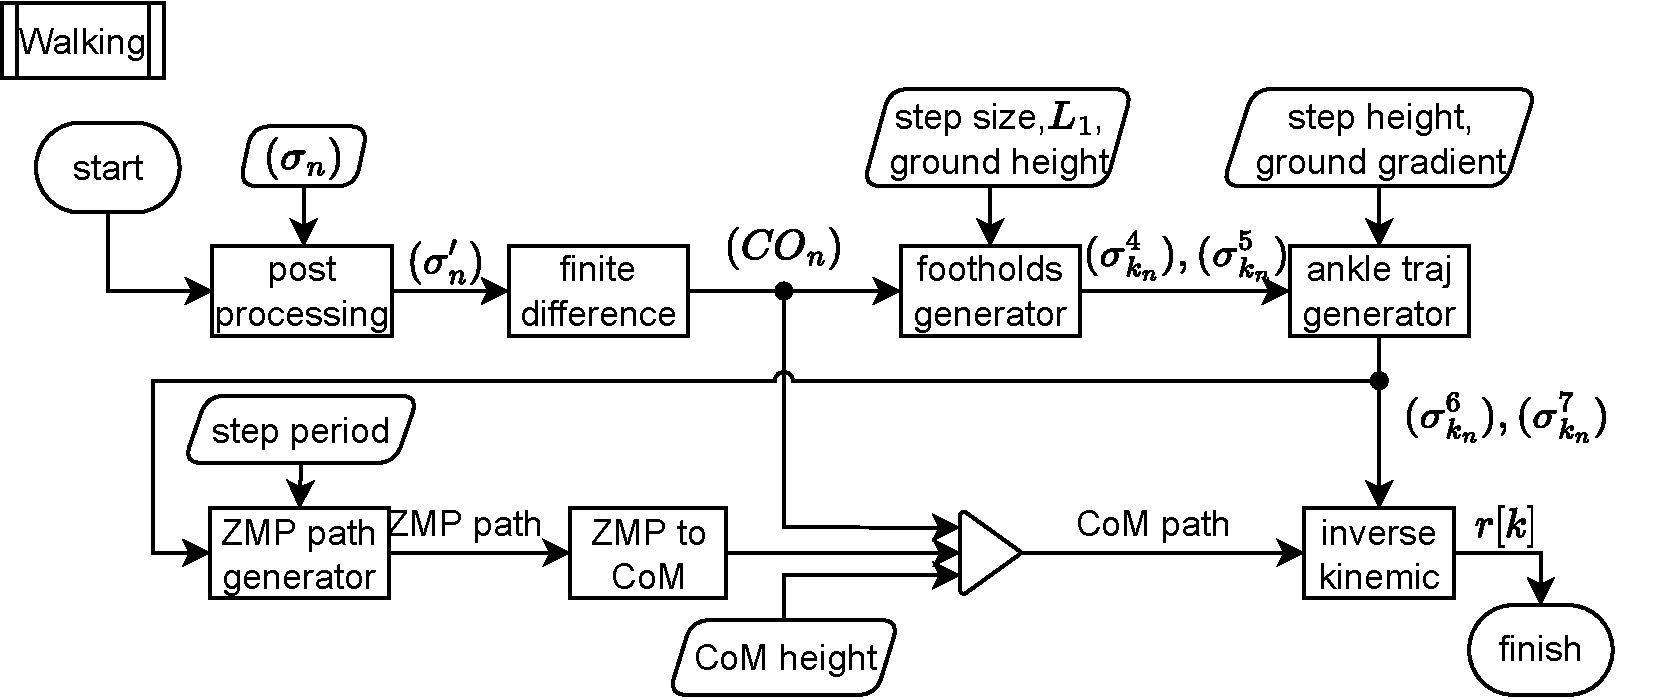
\includegraphics[scale=.3]{fig/walking.pdf}\caption{flowchart of biped robot walking}%
%     \label{fig:walking}
% \end{figure}

Following the same step in UAV, the smoothed path $(\sigma_n')$ for robot can be obtained at first. For ease of explanation, suppose walking is occured between time step $1$ and $N$, i.e., $n\in\mathbb{Z}\cap[1,N]$. Note that $(\sigma_n')$ is not actual CoM reference in robot case since CoM of robot need to "swinging" for balance. Despite that, $(\sigma_n')$ tells the robot the position to go so the forward direction of robot can be obtained by doing finite difference on $(\sigma_n')$ due to the expectation that the robot will move forward (rather than sideways or backward). To keep torso upright, the direction of $\widehat{Z_b}$ is equal to the $z$-axis in the inertial frame $\widehat{Z_g}$. Given $\widehat{X_g}$ and $\widehat{Z_g}$, $\widehat{Y_b}$ can be obtained obviously through cross product. Since the origin of body frame $\{ \widehat{X_g}, \widehat{Y_g}, \widehat{Z_g} \}$ is CoM, the sequence of CoM orientation $(CO_n)$ can be obtained through the above steps.

\begin{remark}
    A frame in $\mathbb{R}^3$ can be determined by given the "position" and "orientation" with respect to a reference frame. That is, given the position and orientation of two joints in a link with known kinematics, the position and orientation of joints between them can be found by IK. Hence, we need to find the  position path and orientation path which compose the desired path.
\end{remark}

Let us denote the $x$ and $y$ component of $\sigma_n'$ in $(\sigma_n')$ as the sequence $(\sigma^{1}_{n}), \sigma^{1}_{n}\in\mathbb{R}^2$. The left and right "envelopes", $(\sigma^{2}_{n})$ and $(\sigma^{3}_{n})$, of $(\sigma^{1}_{n})$ with a fixed distance $L_1$ can be found by $(\sigma^{1}_{n})$ and $(CO_n)$ through the geometric relation between $(\sigma^{i}_{n}), i=1,2,3$, where $L_1$ is feet width (or shoulder width). Then the $x$ and $y$ component of left and right foothold paths, $(\sigma^{2}_{k_n})$ and $(\sigma^{3}_{k_n})$, can be obtained by a given step size, which are the subsequence of $(\sigma^{2}_{n})$ and $(\sigma^{3}_{n})$, respectively. Finally, left and right foothold paths $(\sigma^{i}_{k_n}), \sigma^{i}_{k_n}\in\mathbb{R}^3, i=4,5$ are found by adding $z$ component which is given by ground height.

After foothold paths are obtained, ankle position path can also be obtained by the given step height which is customized by the designer or based on the height of the obstacle to be crossed. Taking the left foothold path as an example, $x$ and $y$ component of the highest position of ankle during stride are set as middle point of two footholds $\sigma^{2}_{k_m}$ and $\sigma^{2}_{k_{m+1}}$ where $m\in\mathbb{Z}\cap[1,N-1]$, and the $z$ component are given by step height. By using spline interpolation, we have the left and right ankle position path $(\sigma^{6}_{n})$ and $(\sigma^{7}_{n})$. The ankle orientation path is found by gradient of ground. Finally, the ankle path is found by combining the position and orientation path together. So far, the remaining work is to find out the CoM path and then to combine with the ankle path to calculate the joint path through IK.

To obtain CoM postion path, ZMP path need to obatin first. ZMP path is obatin through ankle path since ZMP needs to lie in the support face and ankle path point out when a feet is stand on the ground. After that, ZMP path is used to produce CoM postion path by 3D-LIPM as follow:
\begin{equation} \label{eq:LIPM}
    \begin{split}
        & \ddot{x} = \frac{g}{z_c}(x - p_x) \\
        & \ddot{y} = \frac{g}{z_c}(y - p_y)
    \end{split}
\end{equation}
where $(x,y)$ is the position of CoM of the inverted pendulum, $g$ is the gravity acceleration, $z_c$ is the CoM height, and $(p_x,p_y)$ is the position of ZMP. To solve the ODE in (\ref{eq:LIPM}), a method is proposed to convert it to a servo problem \cite{1241826}:
\begin{equation} \label{eq:output tracking}
    \begin{split}
        & \dot{\bar{x}} = A\bar{x} + Bu \\
        & p_x = C\bar{x}
    \end{split}
\end{equation}
where $\bar{x} = \begin{bmatrix}
    x \\ \dot{x} \\ \ddot{x}
\end{bmatrix}$, $A = \begin{bmatrix}
    0 & 1 & 0 \\ 0 & 0 & 1 \\ 0 & 0 & 0
\end{bmatrix}$, $B = \begin{bmatrix}
    0 \\ 0 \\ 1
\end{bmatrix}$, and $C = \begin{bmatrix}
    1 & 0 & -z_c/g
\end{bmatrix}$. Our goal is to find a control input $u$ in order that the output $p_x$ can track a ZMP reference path so that the state variable $x$ is found, which is the CoM position path we want. Unlike conventional methods, the problem is solved by optimal control. The system is discretized first and the discrete LQ tracker is employed to achieve the output tracking. The formulation can be found in TABLE 4.4-1 in \cite{lewis2012optimal}. The CoM position path in the $y$-direction can be found by same procedure since the dynamic of 3D-LIPM in the $x$-direction and $y$-direction is decoupled with same form. 

By combining the CoM position and orientation path, CoM path can be obtained. Finally, the joint path, i.e., reference path $r[k]$ of robot is found by solving IK.

\section{Reference Tracking control}
00
After the reference trajectory is set, the last step is to design a controller for a agent to track it. To analyze the tracking control problem of UAV model in (\ref{eq:uav}) and robot model in (\ref{eq:robot}) together, we represent them by the same form called agent model through some appropriate variable transformations:
\begin{equation} \label{eq:agent} 
    M(x(t))\ddot{x}(t) + H(x(t),\dot{x}(t)) = u(t)
\end{equation}
where $u(t)\in\mathbb{R}^m$ is control input vector, $x(t)\in\mathbb{R}^n$ is state vector, $M(\cdot)\in\mathbb{R}^{n\times n}$ is inertia matrix, and $H(\cdot, \cdot)\in\mathbb{R}^n$ is non-inertial force vector. Suppose the state $x(t)$ is unavailable, i.e., $x(t)$ needs to be obtained by sensor. Besides, its integration $\int_{0}^{t} x(\tau) d\tau$ and differentiation $\dot{x}(t)$ can also be measured by sensor respectively for PID control. Then, the output equation can be formulated as:
\begin{equation} \label{eq:agent output}
    y(t) = C\pmb{x}(t)
\end{equation}
where $y(t)\in\mathbb{R}^l$ is output vector, $C\in\mathbb{R}^{l\times 3n}$ is a known output matrix, and $\pmb{x}(t)=\begin{bmatrix}
    \int_{0}^{t} x^T(\tau) d\tau & x^T(t) & \dot{x}^T(t)
\end{bmatrix}^T$. Futhermore, to make the model more realistic, the following external disturbances encountered in actual scenarios are considered:
\begin{enumerate}
    \item For agent, there exists
    \begin{enumerate*}
        \item coupling effect due to co-channel interference in communication between agents and
        \item cyber-attack on communication network between agents and ground station.
    \end{enumerate*}
    \item For UAV, there exists wind disturbance \cite{9075385}.
    \item For robot, there exists ground reaction force \cite{chen2013human}. 
\end{enumerate}
% \subsubsection{Internal uncertainties}
% In practice, there is uncertaintiey in the parameters of inertia matrix $M$, Coriolis and centripetal force vector $C$, gravitational force vector $G$, and friction vector $F$. Its effect can be expressed as:
% \begin{equation} \label{eq:internal}
%     \begin{split}
%         &M = M_0 + \Delta M, C = C_0 + \Delta C
%         \\
%         &G = G_0 + \Delta G, F = F_0 + \Delta F
%     \end{split}
% \end{equation}
% where $M_0, C_0, G_0$ and  $F_0$ is the nominal part and $\Delta M,\Delta C,\Delta G$ and $\Delta F$ is the uncertain part.
Suppose the above disturbances can be equivalently expressed as the disturbances $d_i(t), i=1,2$ in the nominal model (\ref{eq:agent}) and (\ref{eq:agent output}), the real agent model is given as:
\begin{equation} \label{eq:nonlinear sys} 
    \begin{split}
        & M(x(t))\ddot{x}(t) + H(x(t),\dot{x}(t)) + d_1(t) = u(t)\\
        & y(t) = C\pmb{x}(t) + d_2(t)
    \end{split}
\end{equation}
For designing a tracking controller under unknown external disturbance and making the tracking performance of the agent system (\ref{eq:nonlinear sys}) meet a specified specification, an $H_\infty$ observer-based feedback linearization-based PID(FL-PID) fault tolerance control(FTC) is proposed. Before continuing, the analysis of a linear system version, i.e., after feedback linearization is given first.

\subsection{$H_\infty$ observer-based PID FTC for linear system}
Given a linear system with fault signals:
\begin{equation} \label{eq:4}
    \begin{split}
        & \dot{x}(t)=Ax(t)+B(u(t)+f_1(t)) \\
        & y(t)=Cx(t)+f_2(t)   
    \end{split}  
\end{equation}
where $x(t)\in\mathbb{R}^n$, $u(t)\in\mathbb{R}^m$, $y(t)\in\mathbb{R}^l$, and $f_i:\mathbb{R}\rightarrow \mathbb{R}^{n_i}, f_i(t)\in C^{1}, i=1,2$ with $n_1=m$ and $n_2 = l$.

\textit{
    \begin{remark}
        The fault signal $f_i(t), i=1,2$ are assumed to be smooth rather than bounded, which will make the proposed method more general for practical scenario.
    \end{remark}
}

To deal with the fault signals, an active fault tolerance control is introduced \cite{9306757}. In general, constructing a model for an unknown signal is impossible. However, a smooth model can be used to describe a signal under the smooth assumption. Unlike previous work, a finite-difference-method-based method is proposed to reduce the approximation error between origin fault signal and its smooth model.

From finite difference method, the derivative of the fault signals $\dot{f}_i(t), i=1,2$ with uniform grid $h$ can be expressed as:
\begin{equation} \label{eq:df}
    \dot{f}_i(t)=\sum_{k\in{Z_0}}\frac{a_k f_i(t-kh)}{h} + R_{p-1}(t), Z_0\subset\mathbb{Z}
\end{equation}
where $R_{p-1}(t)\in O(h^{p-1})$ denotes the remainder term, and $p=\vert{Z_0}\vert > 1$ is the accuracy of difference. For constructing a state-space representation, the derivative of $f_i(t-kh),k\in{Z_0}$ in (\ref{eq:df}) is also needed. For the convenience of analysis, let us choose $Z_0=\{ 0,1,\dots,p-1 \}$. Then, we can obtain the following equation by (\ref{eq:df}) by changing index $k$ to $j$:
\begin{equation} \label{eq:df1}
    \dot{f}_i(t-jh)=\sum_{k=0}^{p-1}\frac{a_{j,k} f_i(t-kh)}{h}+\epsilon_j(t), j=0,1,\dots,p-1
\end{equation}
where $\epsilon_j(t)\in O(h^{p-1})$. By arranging $\dot{f}_i(t-jh)$ into a state-space representation, we have:
\begin{equation} \label{eq:7}
    \dot{F}_i(t)=A_iF_i(t)+v_i(t)
\end{equation}
where $v_i(t)=\begin{bmatrix}
    \epsilon_0^T(t) & \epsilon_1^T(t) & \dots & \epsilon_{p-1}^T(t)
\end{bmatrix}^T$, $F_i(t)=\begin{bmatrix}
    f_i^T(t) & f_i^T(t-h) & \dots & f_i^T(t-(p-1)h)
\end{bmatrix}^T$, and $A_i=(a_{j,k})\otimes I_{n_i}$. Then, the fault signals $f_i(t), i=1,2$ are the output of the system in (\ref{eq:7})
\begin{equation} \label{eq:8}
    f_i(t)=C_iF_i(t)
\end{equation}
where $C_i=\begin{bmatrix}
    1 & 0 & \dots & 0
\end{bmatrix}\otimes I_{n_i}$. Sub. (\ref{eq:7}) and (\ref{eq:8}) into (\ref{eq:4}), we get:
\begin{equation} \label{eq:9}
    \begin{split}
        & \dot{\bar{x}} = \bar{A}\bar{x}+\bar{B}u+\bar{v} \\
        & y=\bar{C}\bar{x}
    \end{split}
\end{equation}
where $\bar{x} = \begin{bmatrix}
    x \\ F_1 \\ F_2
\end{bmatrix}$, $\bar{A}=\begin{bmatrix}
    A & BC_1 & 0 \\
    0 & A_1 & 0 \\
    0 & 0 & A_2
\end{bmatrix}$, $\bar{B}=\begin{bmatrix}
    B \\ 0 \\ 0
\end{bmatrix}$, $\bar{C}=\begin{bmatrix}
    C & 0 & C_2
\end{bmatrix}$, and $\bar{v}=\begin{bmatrix}
    0 \\ v_1 \\ v_2
\end{bmatrix}$. Since the fault signals become a state variable of the augment system in (\ref{eq:9}), a Luenberger observer is proposed to estimat them and origin state simutaniously:
\begin{equation} \label{eq:10}
    \begin{split}
        & \dot{\hat{\bar{x}}}=\bar{A}\hat{\bar{x}}+\bar{B}u+{L}(y-\hat{y}) \\
        & \hat{y}=\bar{C}\hat{\bar{x}}  
    \end{split}
\end{equation}
\begin{assumption}
    The augmented system (\ref{eq:9}) is observable.
\end{assumption}
The PID FTC law is given as:
\begin{equation} \label{eq:11}
    u=K\hat{\bar{x}}
\end{equation}
where $K = \begin{bmatrix}
    K_I & K_P & K_D & K_{F_1} & K_{F_2}
\end{bmatrix}$ is total control gain, $K_P,K_I,K_D$ are PID control gain, and $K_{F_i}, i=1,2$ are fault control gain. Let us define the estimation error $\hat{\bar{e}}=\bar{x}-\hat{\bar{x}}$, then an new augmented system can be obtained from (\ref{eq:9}), (\ref{eq:10}) and (\ref{eq:11}):
\begin{equation} \label{eq:aug}
    \dot{\tilde{x}} = \tilde{A}\tilde{x}+\tilde{v}
\end{equation}
where $\tilde{x}=\begin{bmatrix}
    \bar{x} \\ \hat{\bar{e}}
\end{bmatrix}$, $\tilde{A}=\begin{bmatrix}
    \bar{A}+\bar{B}K & -\bar{B}K \\ 0 & \bar{A}+L\bar{C}
\end{bmatrix}$, and $\tilde{v}=\begin{bmatrix}
    \bar{v} \\ 0
\end{bmatrix}$

The tracking control performance below a prescribed disturbance attenuation level $\rho^2$ is given as:
\begin{equation} \label{Hinf}
    H_{\infty}(K, L) = \frac{\int_{0}^{t_f}(\tilde{x}^T(t)Q\tilde{x}(t) + u^T(t)Ru(t))dt - V(\tilde{x}_0)}{\int_{0}^{t_f}\tilde{v}^T(t)\tilde{v}(t)dt}\leq \rho^2 
\end{equation}
where $t_f$ is the final time, $Q > 0$ is the weighting matrix of tracking and estimation error, $R > 0$ is the weighting matrix of control effort, $V(\tilde{x}_0)$ is the initial condition effect on augmented system(\ref{eq:aug}), and $\tilde{v}(t)$ is the total disturbance needs to be attenuated. If we can find the control gain $K$ and observer gain $L$ such that (\ref{Hinf}) holds, then the effect of total disturbance $\tilde{v}(t)$ on tracking and estimation error $\tilde{x}(t)$ can be attenuated to a prescribed level $\rho^2$ from the viewpoint of energy. To find these gains, the following theroem is given.
\begin{theorem} \label{theorem1}
    If
    $$\begin{bmatrix}
        & M_{11} & -\bar{B}Y1 & W_1\sqrt{Q_1} & 0 \\
        & \ast  & M_{22} & 0 & P_2 \\
        & \ast & \ast & -I & 0 \\
        & \ast & \ast & \ast & -\rho^2 
    \end{bmatrix}\leq 0 $$
    where $M_{11}=\bar{A}W_1+\bar{B}Y_1 + (\bar{A}W_1+\bar{B}Y_1)^T + \frac{1}{\rho^1}I$, $M_{22}=P_2\bar{A}+Y_2\bar{C} + (P_2\bar{A}+Y_2\bar{C})^T+Q_2$. Then system (\ref{eq:aug}) achieve $H_\infty$ observer-base stabilized control performance (\ref{Hinf}).
\end{theorem}
\begin{proof}
    proof...
\end{proof}

\subsection{$H_\infty$ observer-based feedback linearization-based PID FTC for agents}
If we can transform the nonlinear system (\ref{eq:nonlinear sys}) to a linear system, the tracking problems for UAV and robot can be solved by Theorem \ref{theorem1}. An feedback linearization-based control law is uesd to solve this issue, which is given as follow:
% To obtain state variable by output measurement, an observer is proposed:
% \begin{equation} \label{eq:nonlinear obs} 
%     \begin{split}
%         & u(t) = M(\hat{x}(t))\ddot{\hat{x}(t)} + H(\hat{x}(t),\dot{\hat{x}(t)})\\
%         & \hat{y}(t) = C\hat{x}(t)
%     \end{split}
% \end{equation}
\begin{equation} \label{eq:control}
    u(t)= M(x_e(t))(\ddot{r}(t) + u_{fb}(t)) + H(x_e(t),\dot{x}_e(t))    
    % & u_{fb} = K_I\int_{0}^{t} e(\tau) d\tau + K_P e(t) + K_D \dot{e}(t) + K_F\hat{F} \\ 
\end{equation}
where $x_e(t)=x(t) + \Delta e(t)$, $\Delta e(t)=e(t)-\hat{e}(t)$ is the error between tracking error $e(t) = x(t) - r(t)\in\mathbb{R}^n$ and estimation of tracking error $\hat{e}(t)$, $u_{fb}(t)$ is feedback control law, and the other term in (\ref{eq:control}) is feed-foward control law for canceling nonlinearity. Substitute (\ref{eq:control}) into state equation (\ref{eq:nonlinear sys}), we get:
\begin{equation}\begin{split} \label{eq:21}
    & M(x_e(t))(\ddot{r}(t) + u_{fb}) + H(x_e(t),\dot{x}_e(t)) \\
    & = M(x(t))\ddot{x}(t) + H(x(t),\dot{x}(t)) + d_1(t)       
\end{split}
\end{equation}
By subtracting $M(x(t))\ddot{r}(t)$ from the left and right sides of (\ref{eq:21}):
\begin{equation} \label{eq:22}
    -\Delta M \ddot{r}(t) + M(x_e(t))u_{fb} = M(x(t))\ddot{e}(t) + \Delta H + d_1(t)
\end{equation}
where $\Delta M = M(x(t)) - M(x_e(t)), \Delta H = H(x(t),\dot{x}(t)) - H(x_e(t),\dot{x}_e(t))$ is the error terms due to difference between true state and estimated state. By Multipling $M(x(t))^{-1}$ from the left and right sides of (\ref{eq:22}) with arrangment, we have:
\begin{equation} \label{eq:23}
    \ddot{e}(t) = u_{fb}(t) + d_3(t)
\end{equation}
where $d_3(t) = -M(x(t))^{-1}(\Delta M(\ddot{r}(t)+u_{fb}) + \Delta H + d_1(t))$. Let $\pmb{e}(t)=\begin{bmatrix}
    \int_{0}^{t}e(\tau)d\tau & e(t) & \dot{e}(t)
\end{bmatrix}\in\mathbb{R}^{3n}$, (\ref{eq:23}) can be rewrited as:
\begin{equation} \label{eq:24}
    \dot{\pmb{e}}(t)=A\pmb{e}(t)+B(u_{fb}(t)+d_3(t))
\end{equation}
where $ A = A_0\otimes I_n, B = B_0\otimes I_n$
with $A_0 = \begin{bmatrix}
    0 & 1 & 0 \\ 0 & 0 & 1 \\ 0 & 0 & 0
\end{bmatrix}, B_0 = \begin{bmatrix}
0 \\ 0 \\ 1
\end{bmatrix} $. Since $C$ is known, we can let $\pmb{y}(t) = y(t) - C\pmb{r}(t)\in\mathbb{R}^{ln}$ where $\pmb{r}(t) = \begin{bmatrix}
    \int_{0}^{t} r^T(\tau) d\tau & r^T(t) & \dot{r}^T(t)
\end{bmatrix}^T$. Then, the output equation in (\ref{eq:nonlinear sys}) can be modified as:
\begin{equation} \label{eq:25}
    \pmb{y}(t) = C\pmb{e}(t) + d_2(t)
\end{equation}
% where $d_4(t) = \Delta C + d_3(t)$ with $\Delta C = C(x(t)-\hat{x}(t))$. 
Combining (\ref{eq:24}) and (\ref{eq:25}), we obtain the linearized system:
\begin{equation} \label{eq:linear sys}
    \begin{split}
        & \dot{\pmb{e}}(t)=A\pmb{e}(t)+B(u_{fb}(t)+d_3(t)) \\
        & \pmb{y}(t)=C\pmb{e}(t)+d_2(t)   
    \end{split}  
\end{equation}
By Theorem \ref{theorem1}, the form show that the system (\ref{eq:nonlinear sys}) can achieve $H_\infty$ performance with the observer
\begin{equation} \label{eq:linear obs}
    \begin{split}
        & \dot{\hat{\bar{e}}}(t)=\bar{A}\hat{\bar{e}}(t) + \bar{B}u_{fb}(t) + L(\pmb{y}(t)-\hat{y}(t)) \\
        & \hat{y}(t)=\bar{C}\hat{\bar{e}}(t)   
    \end{split}  
\end{equation}
and the control law (\ref{eq:control})
where $\hat{\bar{e}}(t)=\begin{bmatrix}
    \hat{\pmb{e}} \\ \hat{F}_1 \\ \hat{F}_2
\end{bmatrix}$, $\hat{\pmb{e}} = \begin{bmatrix}
    \int_{0}^{t} \hat{e}(\tau) d\tau \\ \hat{e}(t) \\ \dot{\hat{e}}(t)
\end{bmatrix}$, $\bar{A}=\begin{bmatrix}
    A & BC_1 & 0 \\
    0 & A_1 & 0 \\
    0 & 0 & A_2
\end{bmatrix}$, $\bar{B}=\begin{bmatrix}
    B \\ 0 \\ 0
\end{bmatrix}$, $\bar{C}=\begin{bmatrix}
    C & 0 & C_2
\end{bmatrix}$, and $u_{fb}=K\hat{\bar{e}}$.
\textit{
    \begin{remark}
        Although the error terms $\Delta e$, $\Delta M$ and $\Delta H$ caused by the difference between state $x(t)$ and estimated state $\hat{x}(t)$ are not necessarily bounded, they can still be estimated as long as they are smooth.
    \end{remark}
}

Although the control gain and observer gain that satisfy the specification can already be found by Theorem \ref{theorem1}, the calculation speed can be further improved by reducing the dimensionality of the system. Since the feedback linearization eliminates the nonlinearity and some degree of coupling of the system (\ref{eq:4}), it can be further split into $n$ subsystems if the output matrix $C$ have the same form to $A$ and $B$, i.e., $C = C_0\otimes I_n$, where $n$ is dimension of state vector and $C_0\in\mathbb{R}^{l\times 3}$.
Due to the fact that $d_3(t)\in\mathbb{R}^n, d_4(t)\in\mathbb{R}^{ln}$, the n subsystems are obtained from (\ref{eq:linear sys}):
\begin{equation} \label{eq:linear subsys}
    \begin{split}
        & \dot{\pmb{e}}_i(t)=A_0\pmb{e}_i(t)+B_0(u_{fd,i}(t)+d_{3,i}(t)) \\
        & \pmb{y}_i(t)=C_0\pmb{e}_i(t)+d_{2,i}(t)   
    \end{split}
\end{equation}
where subscript $i = 1, 2, ..., n$ denote the element in the corresponding vector. By Theorem \ref{theorem1} again, the form show that the subsystems (\ref{eq:linear subsys}) can achieve $H_\infty$ performance. Let $K_i$ be the control gain of subsystems, the origin control gain $K$ of origin agent system can be obtained by $K = \begin{bmatrix}
    \mathit{v}_1 & \mathit{v}_2 & ... & \mathit{v}_n
\end{bmatrix}^T, \mathit{v}_i=K_i\otimes\mathbf{e}_i$ where $\mathbf{e}_i$ is standard unit vectors in $\mathbb{R}^n$. The origin observer gain $L$ can be obtained in the same way. In this case, the calculate speed is improved ...
\textit{
    \begin{remark}
        This method can regard as designing the control and observer gain to each state variable, which is a common control method in practice. However, the gains are not directly adjusted but indirectly designed through prescribed specifications (\ref{Hinf}). Besides, $K_i, i=1,2,\dots,n$ do not have to be the same value (so do $L_i$). Depending on the actual system situation, the appropriate $L_i$ and $K_i$ can be designed for each state variable by adjusting the weighting matrix $Q_i$ and attenuation levels $\rho_i$ for each subsystem.
    \end{remark}
}

\subsection{UAV reference trajectory design and overall flowchart}
Although the design of the agent controller and observer has been completed, the trajectory design of UAV is not done yet. Since the UAV is an underactuated system, the "virtual" control input for UAV $u(t)=\begin{bmatrix}
    f_x & f_y & f_z & \tau_x & \tau_y & \tau_z 
\end{bmatrix}^T\in\mathbb{R}^6$ that obtained from Theorem \ref{theorem1} needs to convert to actual control input $u'(t)=\begin{bmatrix}
    F & \tau_x & \tau_y & \tau_z 
\end{bmatrix}^T\in\mathbb{R}^4$. As the same time, the extra two degrees of freedom are used to find the remaining two reference trajectories $\phi_r(t)$ and $\theta_r(t)$ through inverse dynamics. In simple terms, we want to find a total force $F$ and its angles $\phi_r$, $\theta_r$ and $\psi_r$ from the three component forces $f_x$, $f_y$ and $f_z$. By substituting $\Theta=\begin{bmatrix}
    \phi_r \\ \theta_r \\ \psi_r
\end{bmatrix}$ into $\begin{bmatrix}
        f_x \\ f_y \\ f_z
    \end{bmatrix} = R(\Theta)\begin{bmatrix}
        0 \\ 0 \\ F
\end{bmatrix} $ from UAV dynacmis (\ref{eq:uav}), the 3 unknown variables $F$, $\phi_r$ and $\theta_r$ can be found from these 3 equations because $f_x$, $f_y$, $f_z$ and $\psi_r$ are given.

The overall flowchart of Tracking Control is shown in Fig. \ref{fig:tracking}.

\begin{figure*}[htbp]
    \centering
    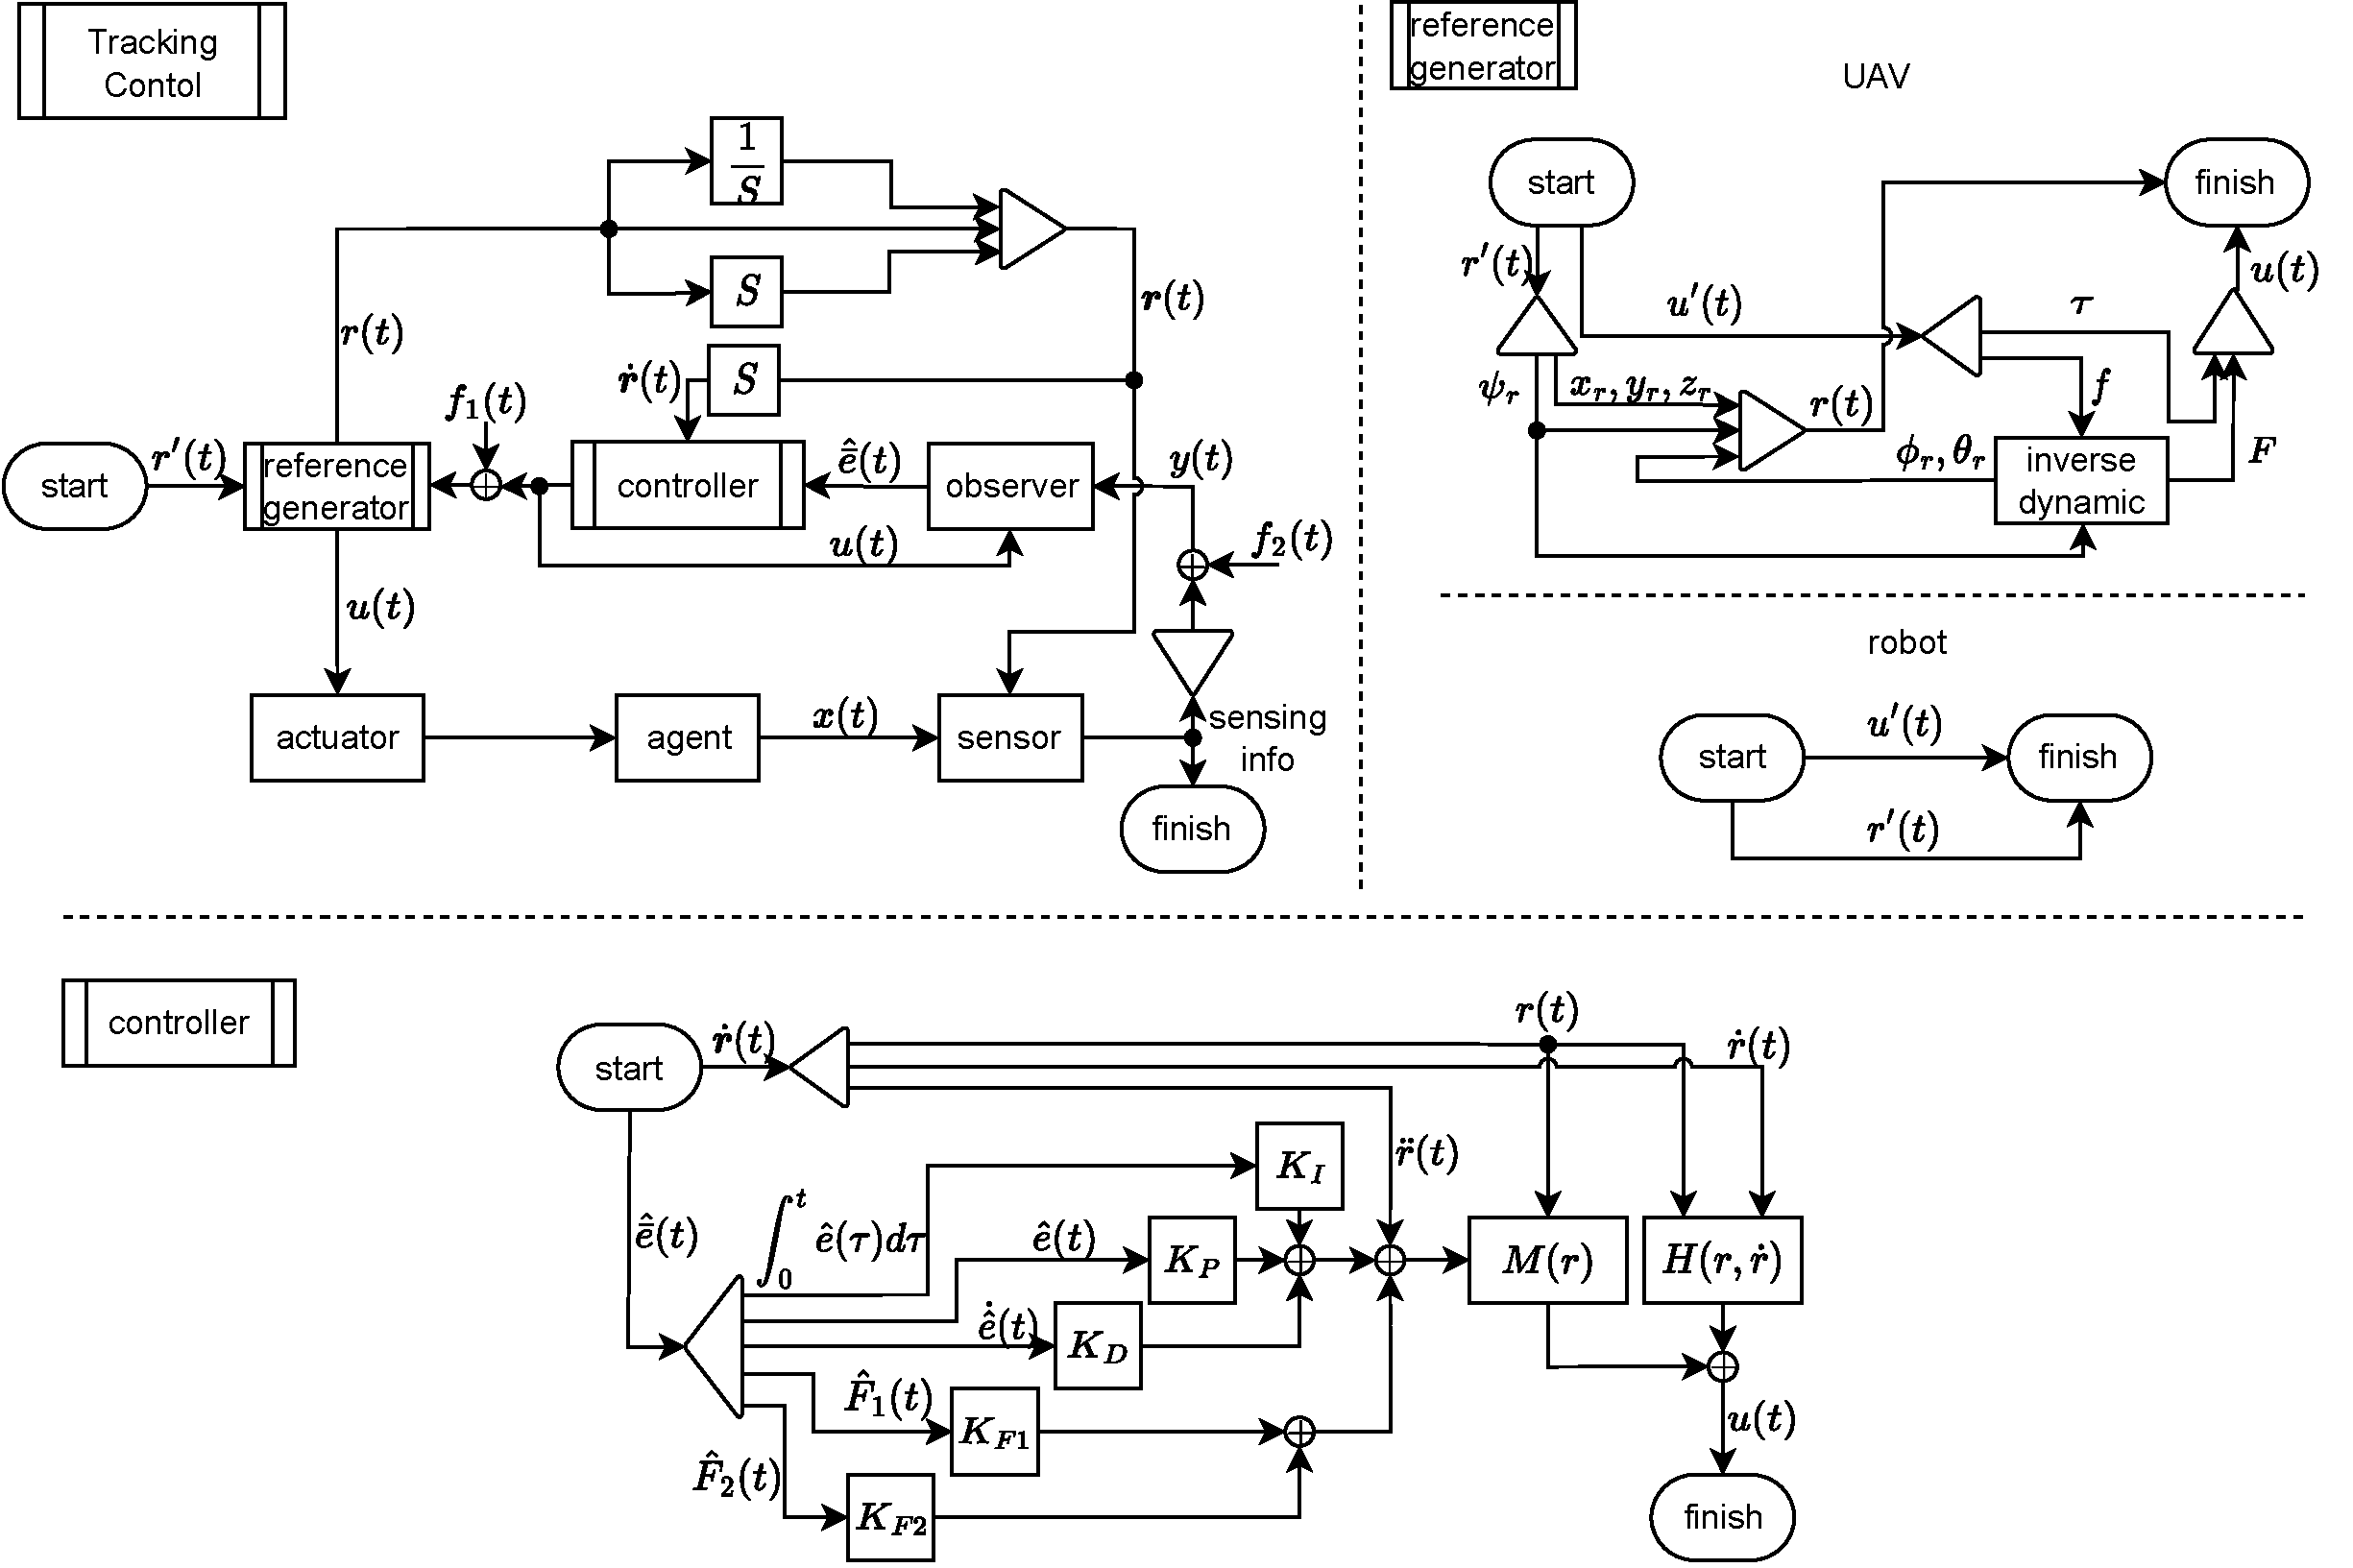
\includegraphics[scale=.5]{fig/tracking.pdf}\caption{flowchart of Tracking Control}%
    \label{fig:tracking}
\end{figure*}

The reference generator for robot is an identity function since it is a fully actuated system. The sensing information includes the agent's own information and environmental info, which is passed back to the high-level block for positioning, mapping and object recognition. Self information is passed to the observer for estimation and tracking error correction.

\section{simulation results}

\section{conclusion}
% \subsection{tracking control of UAV-robot team}
% Since the dynamical system of UAV (\ref{eq:uav}) and robot (\ref{eq:robot}) are nonlinear, it is not easy to design the controller relative to the linear system
% Use feedback linearization, dynamic of UAV and robot become the form (\ref{eq:4})...

% \subsection{reference trajectories design of UAV-robot team}
% \textit{Assumption :} The behavior of uavs and robots is always at "fly" and "walk" respectively during the whole process. 
% \textit{Assumption :} Robots always walking on a flat ground.
% \subsection{path planning of UAV-robot team}
% In order to facilitate the verification of the feasibility of URTS, the following assumptions are given

% \nocite{*}
\bibliographystyle{unsrt}
\bibliography{citation}

\EOD

\end{document}